\documentclass[aspectratio=169]{beamer}
\usetheme{Madrid}
\usecolortheme{default}

% Packages
\usepackage{graphicx}
\usepackage{booktabs}
\usepackage{amsmath}
\usepackage{tikz}

% Title Information
\title[ReConnect Program Impact]{The Economic Impact of Broadband Infrastructure Investment}
\subtitle{Evidence from the USDA ReConnect Program}
\author{Juan Cosme}
\institute{University of South Florida \\ Master of Arts in Economics}
\date{December 11, 2025}

\begin{document}

% Title Slide
\begin{frame}
\titlepage
\end{frame}

%=============================================================================
% SECTION 1: INTRODUCTION
%=============================================================================
\section{Introduction}

\begin{frame}{Motivation}
\begin{itemize}
    \item \textbf{Broadband is essential infrastructure} for 21st century economic development
    \item \textbf{The digital divide:} Before pandemic, 20+ million Americans lacked reliable internet
    \item \textbf{Major policy response:} Infrastructure Investment and Jobs Act (2021)
    \begin{itemize}
        \item \$65 billion allocated for broadband deployment
        \item \$42.45 billion for BEAD program (ongoing)
        \item \$2+ billion through USDA ReConnect (completed projects)
    \end{itemize}
    \item \textbf{Key question:} Do these investments actually improve local economic outcomes?
\end{itemize}
\end{frame}

\begin{frame}{Research Question}
\begin{block}{Main Question}
Did counties receiving ReConnect broadband funding achieve better economic outcomes than similar counties without funding?
\end{block}

\vspace{0.5cm}

\textbf{Focus:}
\begin{itemize}
    \item 959 counties across 10 states
    \item Time period: 2019 (pre) to 2022-2023 (post)
    \item Main outcomes: Employment and household income
    \item Method: Difference-in-differences
\end{itemize}
\end{frame}

\begin{frame}{Preview of Main Finding}
\begin{alertblock}{Surprising Result}
ReConnect funding led to a \textbf{statistically significant reduction} of 764 jobs in treated counties relative to controls (p $<$ 0.01)
\end{alertblock}

\vspace{0.5cm}

\textbf{But what does this mean?}
\begin{itemize}
    \item Not absolute job losses!
    \item Treated counties grew \textbf{slower} than controls
    \item Control counties: +4.2\% employment growth
    \item Treated counties: +2.6\% employment growth
    \item Suggests short-run adjustment costs
\end{itemize}
\end{frame}

%=============================================================================
% SECTION 2: DATA & METHODS
%=============================================================================
\section{Data \& Methods}

\begin{frame}{The ReConnect Program}
\textbf{USDA ReConnect Program (launched 2019):}
\begin{itemize}
    \item Provides grants and loans for rural broadband infrastructure
    \item Targets areas lacking sufficient internet access ($<$ 25 Mbps)
    \item Awards announced 2019-2022, deployment 2020-2023
    \item Over \$2 billion awarded to rural communities
\end{itemize}



\vspace{0.3cm}

\textbf{Policy Relevance:}
\begin{itemize}
    \item ReConnect shares design features with BEAD program
    \item Both prioritize unserved rural areas
    \item Evidence from ReConnect informs \$42.45 billion BEAD deployment
\end{itemize}
\end{frame}

\begin{frame}{Data Sources}
\begin{table}
\small
\begin{tabular}{ll}
\toprule
\textbf{Variable} & \textbf{Source} \\
\midrule
Employment & BLS Quarterly Census of Employment \& Wages \\
 & (QCEW) - covers 95\% of all jobs \\
\addlinespace
Income & Census American Community Survey (ACS) \\
 & Limited to 114 counties (data availability) \\
\addlinespace
Treatment & USDA ReConnect award announcements \\
 & 2019-2022 funding rounds \\
\addlinespace
Rural Status & USDA Rural-Urban Continuum Codes (RUCC) \\
\bottomrule
\end{tabular}
\end{table}

\vspace{0.3cm}

\textbf{Final Sample:}
\begin{itemize}
    \item 959 counties in 10 states (VA, NC, GA, TN, KY, MI, WI, MN, MT, ID)
    \item 122 treated, 837 control counties
    \item 3 time periods: 2019, 2022, 2023
\end{itemize}
\end{frame}

\begin{frame}{Empirical Strategy: Difference-in-Differences}
\textbf{Basic DiD Specification:}

\begin{equation*}
Y_{it} = \alpha_i + \lambda_t + \beta \cdot (\text{Treated}_i \times \text{Post}_t) + \varepsilon_{it}
\end{equation*}



\vspace{0.3cm}

\textbf{Where:}
\begin{itemize}
    \item $Y_{it}$ = Employment (or income) in county $i$, year $t$
    \item $\alpha_i$ = County fixed effects (control time-invariant differences)
    \item $\lambda_t$ = Year fixed effects (control common time trends)
    \item $\beta$ = \textbf{Treatment effect} (our coefficient of interest)
\end{itemize}



\vspace{0.3cm}

\textbf{Standard errors:} Clustered at county level
\end{frame}

\begin{frame}{Key Identification Assumption: Parallel Trends}
\begin{block}{Parallel Trends Assumption}
In the absence of treatment, treated and control counties would have experienced the same employment trends
\end{block}



\vspace{0.3cm}

\textbf{How we test this:}
\begin{enumerate}
    \item Visual inspection of pre-treatment trends (Figure 1)
    \item Event study showing no effects in 2019
    \item Baseline balance tests (Table 8)
\end{enumerate}



\vspace{0.3cm}

\textbf{Limitation:} Only one pre-treatment period (2019)
\begin{itemize}
    \item ReConnect started in 2019 - can't use earlier years
    \item Rely on visual evidence and baseline balance
\end{itemize}
\end{frame}

%=============================================================================
% SECTION 3: DATA DESCRIPTION & IDENTIFICATION
%=============================================================================
\section{Data \& Identification}

\begin{frame}{Summary Statistics (2019 Baseline)}
\begin{table}
\footnotesize
\begin{tabular}{lcccccc}
\toprule
 & \multicolumn{3}{c}{\textbf{Control (N=837)}} & \multicolumn{3}{c}{\textbf{Treated (N=122)}} \\
\cmidrule(lr){2-4} \cmidrule(lr){5-7}
\textbf{Variable} & Mean & Std. Dev. & N & Mean & Std. Dev. & N \\
\midrule
Total Employment & 32,864 & 87,776 & 837 & 14,300 & 25,073 & 122 \\
Median HH Income & \$76,513 & \$16,871 & 294 & \$76,551 & \$8,533 & 29 \\
Establishments & 2,099 & 5,935 & 837 & 962 & 1,733 & 122 \\
Rural (RUCC $\geq$ 4) & 0.579 & 0.494 & 837 & 0.746 & 0.437 & 122 \\
\bottomrule
\end{tabular}
\end{table}

\vspace{0.3cm}

\textbf{Key observations:}
\begin{itemize}
    \item Treated counties significantly smaller (14,300 vs. 32,864 employees)
    \item More rural (75\% vs. 58\% rural)
    \item \textbf{Similar income levels} (\$76,551 vs. \$76,513) - no systematic economic differences
    \item County fixed effects will control for size and rural status
\end{itemize}
\end{frame}

\begin{frame}{Visual Evidence: Parallel Trends (Employment)}
\begin{center}
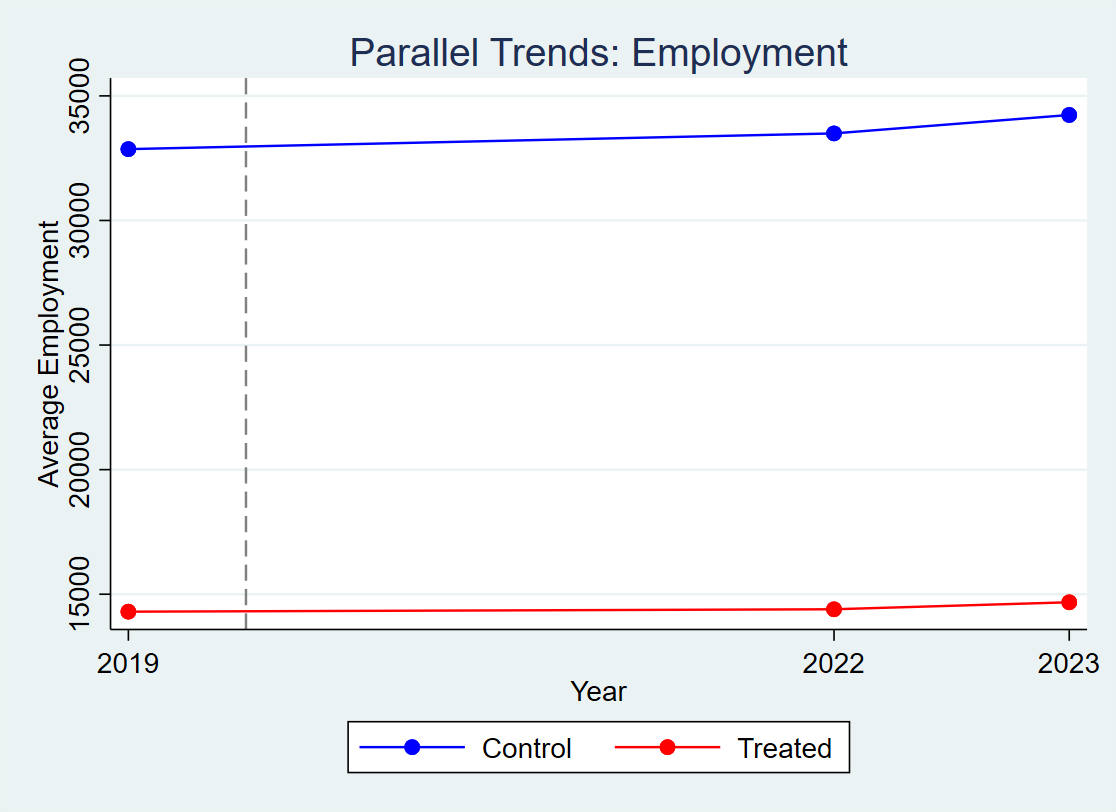
\includegraphics[width=0.75\textwidth]{fig_parallel_trends_employment.png}
\end{center}

\vspace{0.3cm}

\textbf{Critical for identification:} Both groups show flat trends in 2019 (pre-treatment), then diverge after treatment begins. This supports the parallel trends assumption necessary for causal interpretation.
\end{frame}

%=============================================================================
% SECTION 4: RESULTS
%=============================================================================
\section{Main Results}

\begin{frame}{Main Result: Employment Effects}
\begin{table}
\footnotesize
\begin{tabular}{lcccc}
\toprule
 & \textbf{(1)} & \textbf{(2)} & \textbf{(3)} & \textbf{(4)} \\
 & Basic & w/ Rural & State-Year FE & Log Spec \\
\midrule
Treatment $\times$ Post & -763.92*** & -763.92*** & 1785.04 & -0.0062 \\
 & (278.91) & (278.91) & (1838.27) & (0.0075) \\
\addlinespace
Observations & 2,877 & 2,877 & 318 & 2,877 \\
Adjusted R$^2$ & 0.998 & 0.998 & 0.999 & 0.999 \\
\bottomrule
\end{tabular}
\end{table}

\vspace{0.3cm}

\textbf{Interpretation of Column (1):}
\begin{itemize}
    \item \textbf{764 fewer jobs} in treated counties (p = 0.006)
    \item Represents 5.3\% reduction relative to baseline
    \item Highly statistically significant at 1\% level
\end{itemize}
\end{frame}

\begin{frame}{What Does ``Negative Effect'' Mean?}
\begin{table}
\footnotesize
\begin{tabular}{lccc}
\toprule
\textbf{Year} & \textbf{Control Avg} & \textbf{Treated Avg} & \textbf{Difference} \\
\midrule
2019 & 32,864 & 14,300 & 18,564 \\
2022 & 33,495 & 14,396 & 19,099 \\
2023 & 34,234 & 14,678 & 19,556 \\
\addlinespace
\textbf{Growth} & \textbf{+1,370 (+4.2\%)} & \textbf{+378 (+2.6\%)} & \textbf{Gap +992} \\
\bottomrule
\end{tabular}
\end{table}



\vspace{0.3cm}

\begin{alertblock}{Critical Insight}
\textbf{Not absolute job losses!} Both groups added jobs, but treated counties grew more slowly than controls. The negative effect represents \textbf{slower employment growth}, not economic collapse.
\end{alertblock}
\end{frame}

\begin{frame}{Event Study: Effects Over Time}
\begin{columns}
\begin{column}{0.5\textwidth}
\begin{table}
\footnotesize
\begin{tabular}{lc}
\toprule
\textbf{Year} & \textbf{Effect} \\
\midrule
2022 & -535** \\
 & (253) \\
2023 & -993*** \\
 & (310) \\
\bottomrule
\end{tabular}
\end{table}

\vspace{0.3cm}

\textbf{Key findings:}
\begin{itemize}
    \item Effect appears immediately (2022)
    \item Effect \textbf{grows} over time
    \item Nearly doubles by 2023
\end{itemize}
\end{column}

\begin{column}{0.5\textwidth}
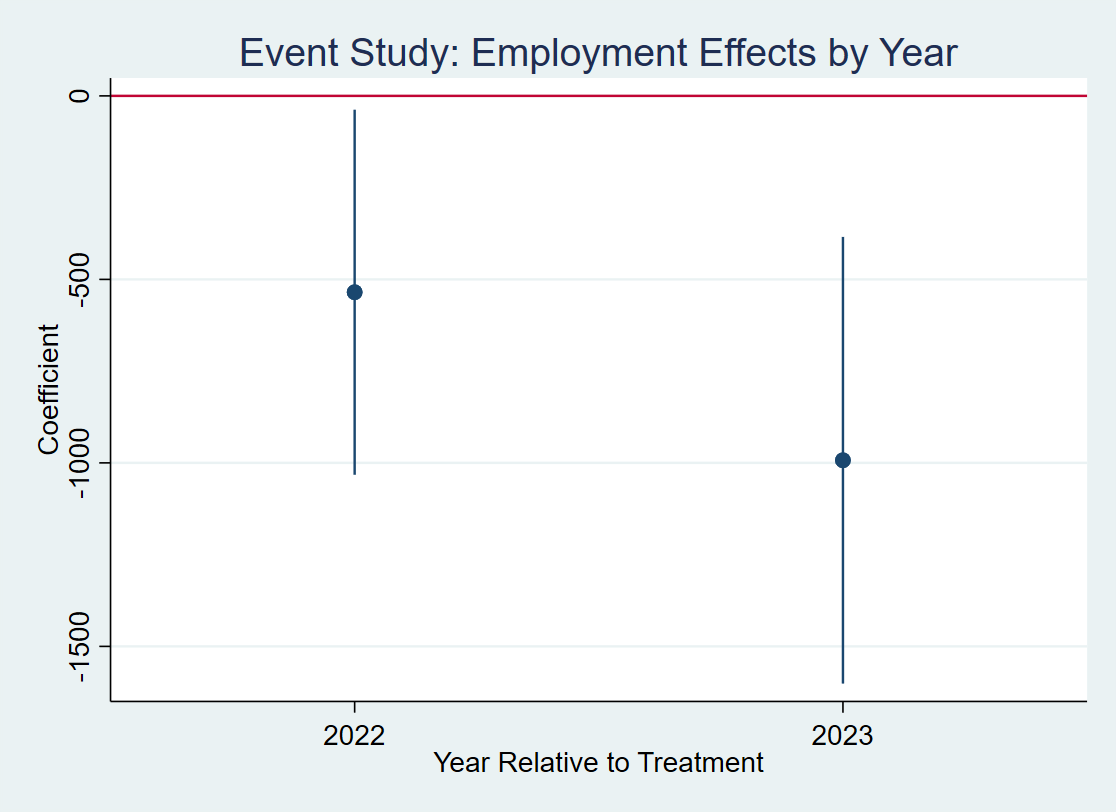
\includegraphics[width=\textwidth]{fig_event_study_employment.png}
\end{column}
\end{columns}

\vspace{0.3cm}

\textbf{Interpretation:} Cumulative impact as more households adopt broadband and behavioral adjustments occur
\end{frame}

\begin{frame}{Income Effects}
\begin{table}
\footnotesize
\begin{tabular}{lcccc}
\toprule
 & \textbf{(1)} & \textbf{(2)} & \textbf{(3)} & \textbf{(4)} \\
 & Basic & w/ Rural & State-Year FE & Log Spec \\
\midrule
Treatment $\times$ Post & 97.63 & 97.63 & 1.97 & 0.0023 \\
 & (945.43) & (945.43) & (1212.79) & (0.0138) \\
\addlinespace
Observations & 323 & 323 & 318 & 323 \\
Counties & 114 & 114 & 112 & 114 \\
\bottomrule
\end{tabular}
\end{table}

\vspace{0.3cm}

\textbf{Interpretation:}
\begin{itemize}
    \item Small effect (+\$98), not statistically significant
    \item Sample limited to 114 counties - reduced power
    \item Suggests no detectable income impact
    \item Consistent with job displacement (residents keep income via remote work)
\end{itemize}
\end{frame}

\begin{frame}{Heterogeneity: Rural vs. Urban Counties}
\begin{table}
\footnotesize
\begin{tabular}{lcc}
\toprule
 & \textbf{Employment} & \textbf{Income} \\
\midrule
Treatment $\times$ Post $\times$ Rural & -969.60*** & 465.18 \\
 & (240.70) & (455.25) \\
\addlinespace
Treatment $\times$ Post $\times$ Urban & -160.16 & 20.23 \\
 & (601.84) & (1102.32) \\
\addlinespace
Test: Rural = Urban (p-value) & 0.145 & 0.659 \\
\bottomrule
\end{tabular}
\end{table}

\vspace{0.3cm}

\textbf{Key finding:}
\begin{itemize}
    \item \textbf{Negative effect concentrated in rural counties}
    \item Rural: -970 jobs (highly significant)
    \item Urban: -160 jobs (not significant)
    \item Suggests rural labor markets more vulnerable to displacement
\end{itemize}
\end{frame}

\begin{frame}{Robustness Checks}
\begin{table}
\footnotesize
\begin{tabular}{lcccc}
\toprule
 & \textbf{Drop} & \textbf{State} & \textbf{Common} & \textbf{Establish-} \\
 & \textbf{Outliers} & \textbf{Cluster} & \textbf{Sample} & \textbf{ments} \\
\midrule
Treatment $\times$ Post & -394* & -404 & -404 & -332*** \\
 & (226) & (2399) & (2624) & (70) \\
\addlinespace
Observations & 2,598 & 323 & 323 & 2,877 \\
\bottomrule
\end{tabular}
\end{table}

\vspace{0.3cm}

\textbf{Interpretation:}
\begin{itemize}
    \item Consistently negative across specifications
    \item \textbf{Establishments also declined} (-332, highly significant)
    \item Not just employment - businesses closing too
    \item Results robust to outliers, clustering, sample restrictions
\end{itemize}
\end{frame}

%=============================================================================
% SECTION 5: DISCUSSION
%=============================================================================
\section{Discussion}

\begin{frame}{Why Negative Employment Effects?}
\textbf{Four potential mechanisms:}

\begin{enumerate}
    \item \textbf{Remote Work Displacement}
    \begin{itemize}
        \item Broadband enables residents to work remotely for firms outside county
        \item Measured employment falls even though residents remain employed
        \item Especially plausible in rural areas with limited local options
    \end{itemize}
    
    
    
    \item \textbf{Short-Run Disruption}
    \begin{itemize}
        \item Infrastructure construction temporarily disrupts businesses
        \item But growing effects over time somewhat inconsistent with this
    \end{itemize}
    
    
    
    \item \textbf{Sectoral Reallocation (Creative Destruction)}
    \begin{itemize}
        \item Broadband enables e-commerce, displacing brick-and-mortar retail
        \item Traditional jobs disappear quickly, new digital jobs emerge slowly
        \item Net effect negative in short run
    \end{itemize}
    
    
    
    \item \textbf{Selection and Pre-Existing Trends}
    \begin{itemize}
        \item ReConnect may have targeted declining counties
        \item But parallel trends evidence argues against this
    \end{itemize}
\end{enumerate}

\vspace{0.2cm}

\textbf{Most likely:} Combination of remote work displacement and sectoral reallocation
\end{frame}

\begin{frame}{Policy Implications}
\textbf{Key takeaways for policymakers:}

\begin{enumerate}
    \item \textbf{Don't assume automatic positive effects}
    \begin{itemize}
        \item Infrastructure investment $\neq$ guaranteed local job growth
        \item Short-run adjustment costs are real
    \end{itemize}
    
    
    
    \item \textbf{Need complementary policies}
    \begin{itemize}
        \item Workforce development programs
        \item Support for businesses adapting to digital economy
    \end{itemize}
    
    
    
    \item \textbf{Rural areas require different approaches}
    \begin{itemize}
        \item Effects concentrated in rural counties
        \item Need targeted interventions for rural labor markets
    \end{itemize}
    
    
    
    \item \textbf{Long-run evaluation needed}
    \begin{itemize}
        \item Effects may be temporary (1-4 years observed)
        \item Positive effects might emerge over 5-10 years
    \end{itemize}
    
    
    
    \item \textbf{Implications for \$42.45B BEAD Program}
    \begin{itemize}
        \item Anticipate short-run adjustment costs
        \item Plan complementary workforce and business support
    \end{itemize}
\end{enumerate}
\end{frame}

\begin{frame}{Limitations}
\textbf{Key limitations to acknowledge:}

\begin{enumerate}
    \item \textbf{Limited time periods}
    \begin{itemize}
        \item Only 2019, 2022, 2023 observed
        \item Can't test pre-trends with multiple pre-periods
    \end{itemize}
    
    
    
    \item \textbf{Income data limited}
    \begin{itemize}
        \item Only 114 of 959 counties have income data
    \end{itemize}
    
    
    
    \item \textbf{Couldn't test all proposed mechanisms}
    \begin{itemize}
        \item Wanted deployment vs. adoption - lacked data
        \item Wanted sector-specific effects - data unavailable
    \end{itemize}
    
    
    
    \item \textbf{Can't observe actual broadband deployment timing}
    \begin{itemize}
        \item Treatment based on award dates
        \item Actual deployment may lag 12-24 months
    \end{itemize}
    
    
    
    \item \textbf{Can't distinguish job losses from remote work shifts}
    \begin{itemize}
        \item County data counts jobs by workplace location
        \item Complicates welfare interpretation
    \end{itemize}
\end{enumerate}

\vspace{0.2cm}

\textbf{Despite limitations:} DiD design is sound, results are robust, findings are policy-relevant
\end{frame}

%=============================================================================
% SECTION 6: CONCLUSION
%=============================================================================
\section{Conclusion}

\begin{frame}{Summary of Contributions}
\textbf{This paper contributes to literature in three ways:}

\begin{enumerate}
    \item \textbf{Rigorous causal estimates of ReConnect}
    \begin{itemize}
        \item Quasi-experimental DiD methodology
        \item 959 counties across 10 states, 2019-2023
        \item Evidence directly relevant for \$42.45B BEAD program
    \end{itemize}
    
    
    
    \item \textbf{Documents unexpected negative short-run effects}
    \begin{itemize}
        \item 764 fewer jobs in treated counties (slower growth)
        \item Highlights adjustment costs often ignored in policy debates
        \item Suggests need for complementary policies
    \end{itemize}
    
    
    
    \item \textbf{Demonstrates heterogeneous effects}
    \begin{itemize}
        \item Effects concentrated in rural counties (-970 vs. -160)
        \item Broadband's impact depends on local economic conditions
        \item Rural areas need different policy approaches
    \end{itemize}
\end{enumerate}
\end{frame}

\begin{frame}{Main Takeaway}
\begin{block}{Key Message}
Broadband infrastructure investment does \textbf{not automatically generate local employment gains}. The path from infrastructure to economic development is complex, with potential short-run adjustment costs that policymakers must anticipate and address.
\end{block}



\vspace{0.5cm}

\textbf{Implications for \$65 billion in federal broadband funding:}
\begin{itemize}
    \item Plan for transition costs
    \item Implement complementary workforce development
    \item Tailor policies to rural vs. urban contexts
    \item Monitor long-run outcomes (5-10 years)
    \item Don't expect immediate job creation
\end{itemize}
\end{frame}

\begin{frame}{Future Research}
\textbf{Important directions for future work:}

\begin{enumerate}
    \item \textbf{Longer time horizons}
    \begin{itemize}
        \item Track ReConnect counties over 5-10 years
        \item Test if negative effects reverse in long run
    \end{itemize}
    
    
    
    \item \textbf{Worker-level data}
    \begin{itemize}
        \item Distinguish job losses from remote work shifts
        \item Better welfare interpretation
    \end{itemize}
    
    
    
    \item \textbf{Sector-specific analysis}
    \begin{itemize}
        \item Which industries most affected?
        \item Test retail vs. professional services vs. manufacturing
    \end{itemize}
    
    
    
    \item \textbf{Deployment vs. adoption mechanisms}
    \begin{itemize}
        \item Does infrastructure alone drive effects?
        \item Major policy implications for subsidies
    \end{itemize}
    
    
    
    \item \textbf{Complementary policies}
    \begin{itemize}
        \item Test effectiveness of workforce development programs
        \item Identify best practices for minimizing adjustment costs
    \end{itemize}
\end{enumerate}
\end{frame}

%=============================================================================
% FINAL SLIDE
%=============================================================================

\begin{frame}[plain,c]
\begin{center}
\Huge Questions?
\end{center}
\end{frame}

%=============================================================================
% BACKUP SLIDES
%=============================================================================

\appendix

\begin{frame}[noframenumbering]{Backup: Income Parallel Trends}
\begin{center}
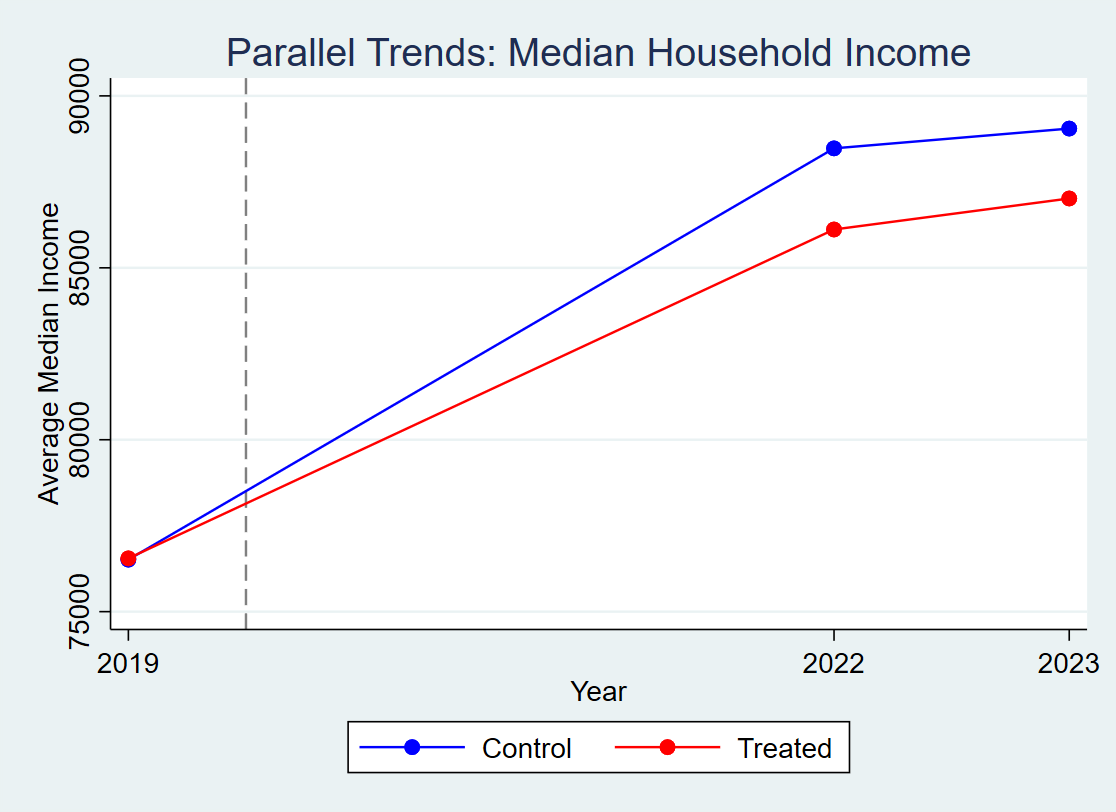
\includegraphics[width=0.7\textwidth]{fig_parallel_trends_income.png}
\end{center}

\vspace{0.3cm}

\textbf{Note:} Both groups trending upward. Limited to 114 counties with available income data. No clear treatment effect visible.
\end{frame}

\begin{frame}[noframenumbering]{Backup: Full Regression Output}
\begin{table}
\tiny
\begin{tabular}{lcccc}
\toprule
 & \textbf{(1)} & \textbf{(2)} & \textbf{(3)} & \textbf{(4)} \\
 & Basic & w/ Rural & State-Year FE & Log Spec \\
\midrule
Treatment $\times$ Post & -763.92*** & -763.92*** & 1785.04 & -0.0062 \\
 & (278.91) & (278.91) & (1838.27) & (0.0075) \\
\addlinespace
County FE & Yes & Yes & Yes & Yes \\
Year FE & Yes & Yes & No & Yes \\
State $\times$ Year FE & No & No & Yes & No \\
\addlinespace
Observations & 2,877 & 2,877 & 318 & 2,877 \\
Adjusted R$^2$ & 0.998 & 0.998 & 0.999 & 0.999 \\
Clusters (counties) & 959 & 959 & 112 & 959 \\
\bottomrule
\end{tabular}
\end{table}

\vspace{0.2cm}

\footnotesize
\textbf{Notes:} Dependent variable is total county employment (Columns 1-3) or log employment (Column 4). Standard errors clustered at county level. *** p$<$0.01, ** p$<$0.05, * p$<$0.10.
\end{frame}

\end{document}